\section{Methodology}
\label{sec:method}

In this section, we detail the architectural components of \method. The overarching framework is depicted in Figure~\ref{fig:pipeline}. \method operates in a purely training-free manner across the multi-stage diffusion process, combining attention-level orthogonal feature decomposition, temporal Sigmoid scheduling, score-orthogonal gradient guidance on the latent manifold, and early-step clean-latent statistical pushforward.

\begin{figure*}[t]
\centering
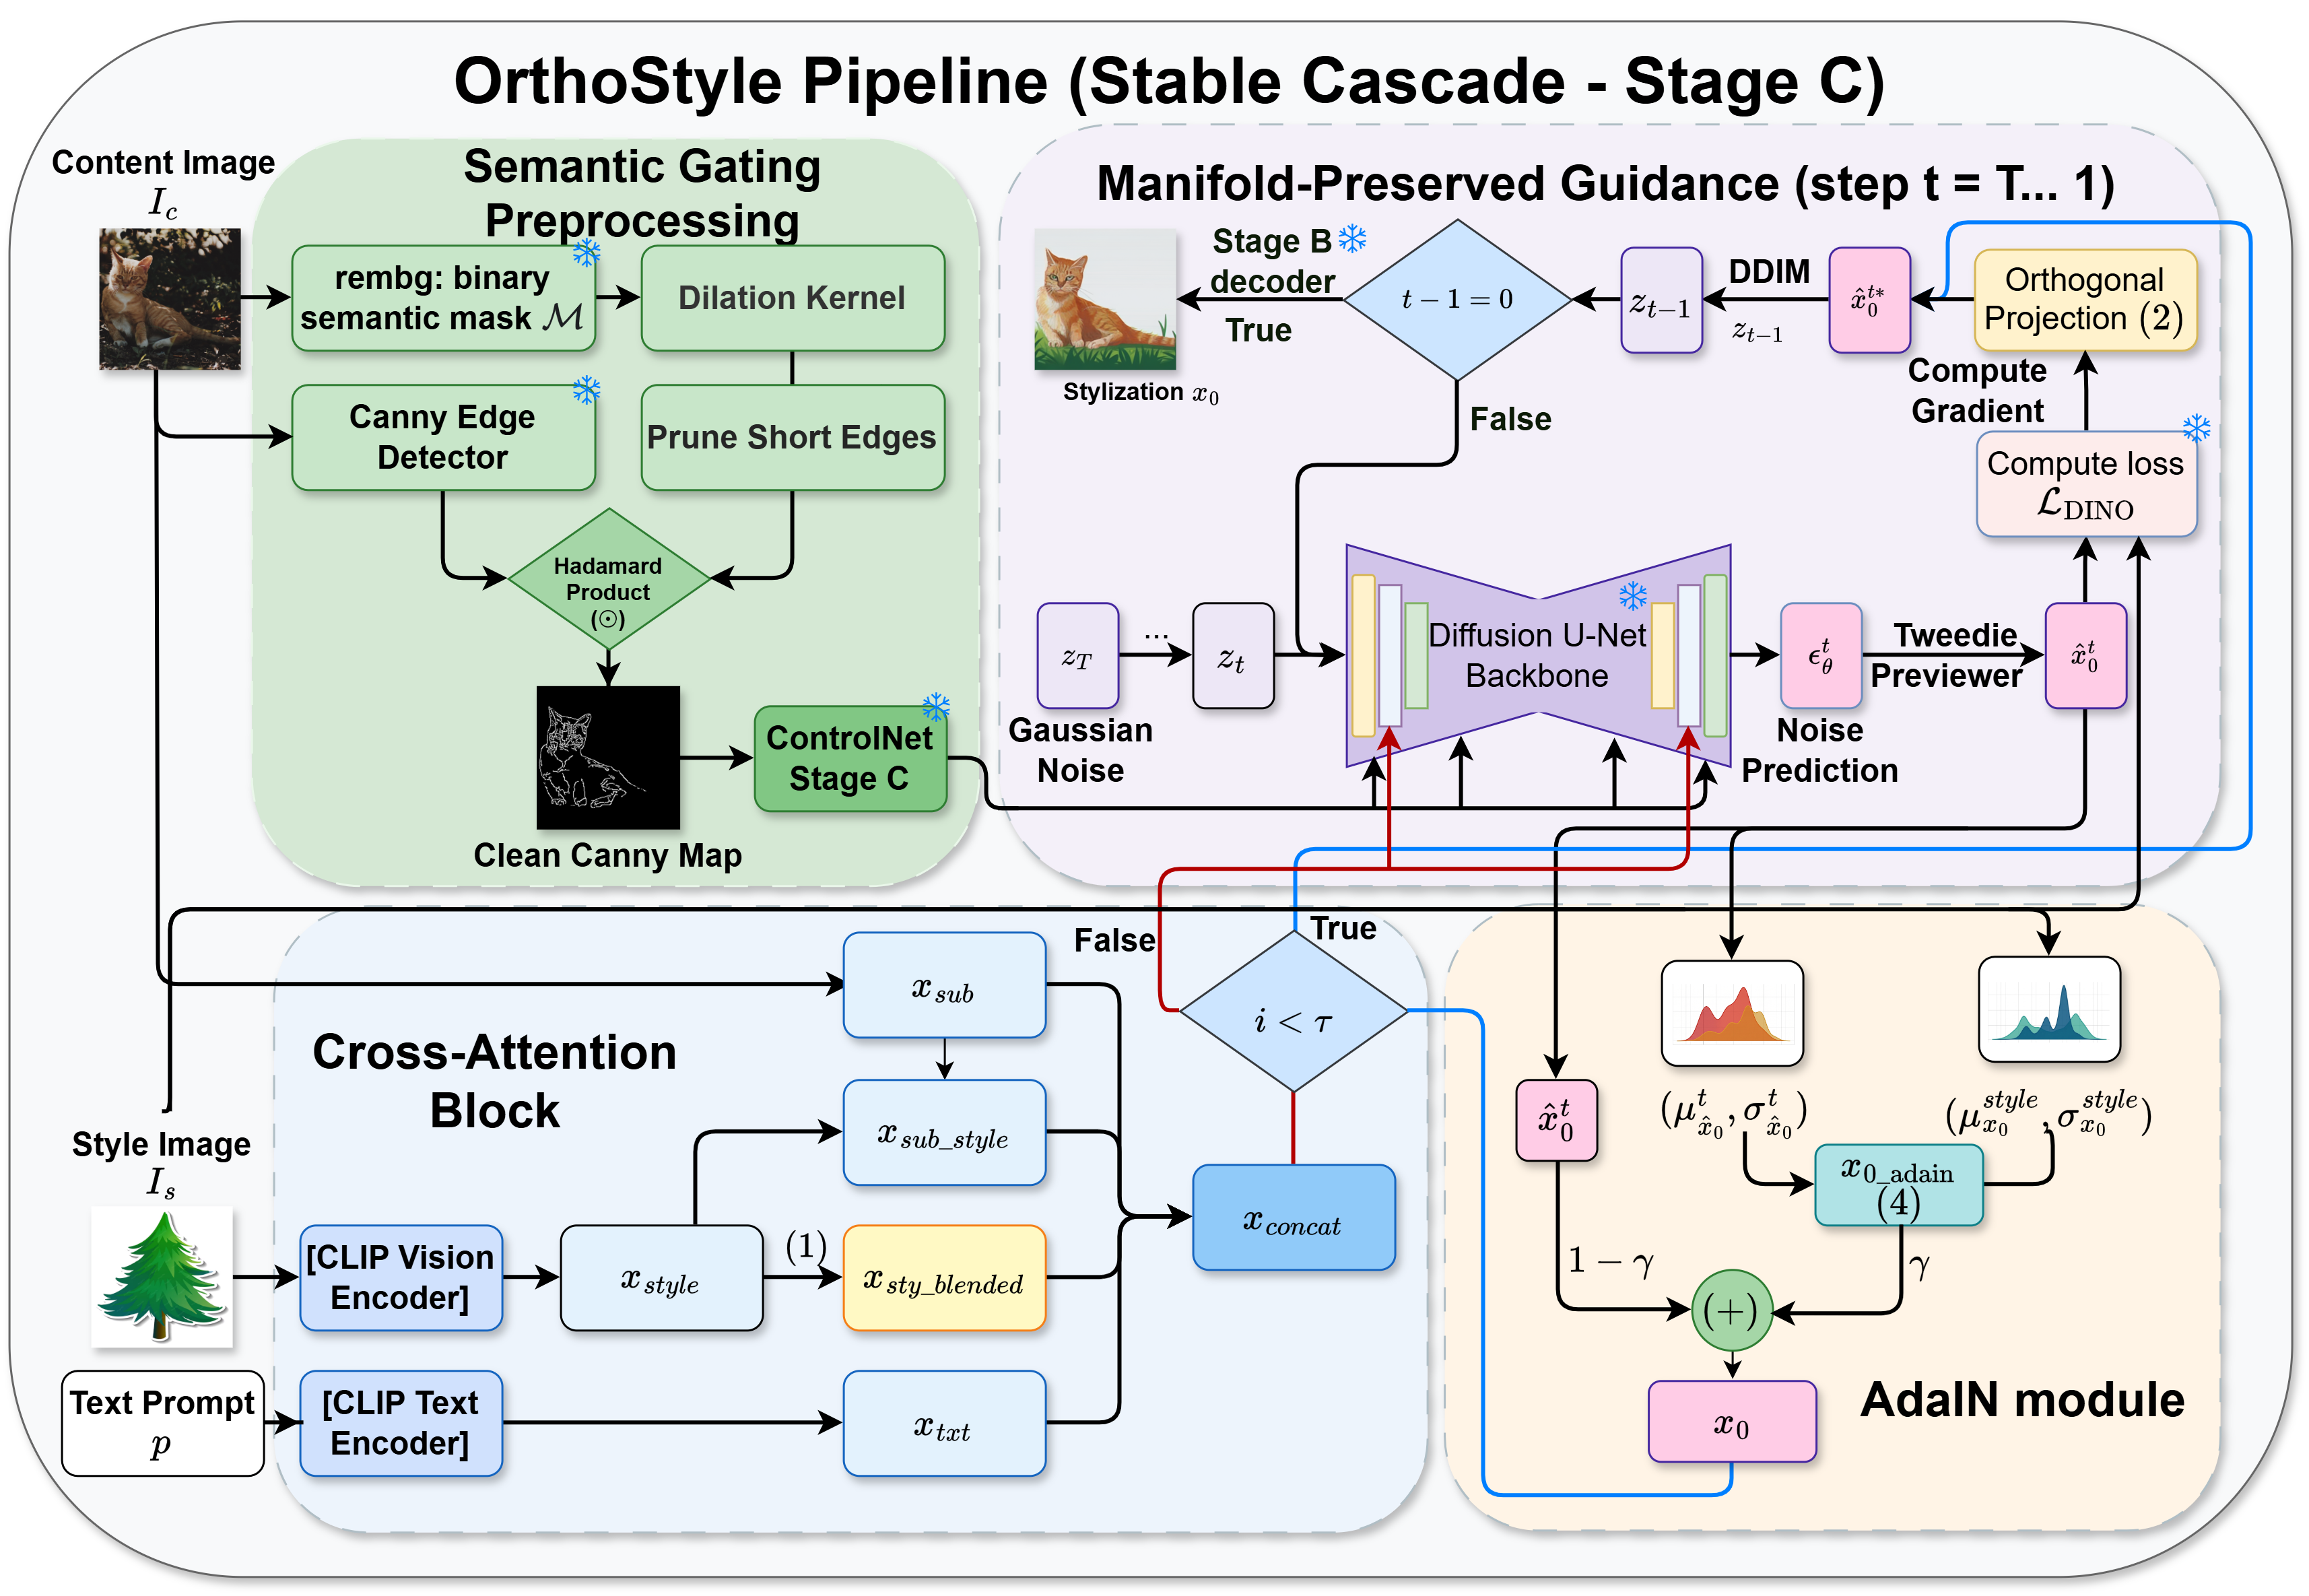
\includegraphics[width=\textwidth]{figs/pipeline.png}
\caption{\textbf{Comprehensive Pipeline of \method.} (Top) Cross-attention layers decouple content and style into orthogonal subspaces with energy compensation. (Bottom) During reverse diffusion, DINO-ViT terminal guidance computes score-orthogonal gradients to navigate the valid data manifold, assisted by early-stage clean latent AdaIN pushforward and semantic Canny structural gating.}
\label{fig:pipeline}
\end{figure*}

\subsection{Multi-Stream Cross-Attention Decomposition}
\label{subsec:attn_decomp}
Let $\bx \in \R^{B \times (H \cdot W) \times C}$ be the intermediate spatial query representations within an attention block of the generator, and $\mathbf{kv} \in \R^{B \times L \times C}$ denote the concatenated key-value tokens containing both text embeddings and visual CLIP prefix tokens of length $L_{\text{clip}}$.

Instead of computing a single entangled attention output, \method decomposes the conditioning stream into four distinct semantic components:
\begin{enumerate}
    \item \textbf{Text Stream} ($\xtxt$): Attends purely to text prompt tokens $\mathbf{kv}_{:\,-2L_{\text{clip}}}$, ensuring conceptual prompt grounding.
    \item \textbf{Subject Stream} ($\xsub$): Attends to the reference content/subject tokens $\mathbf{kv}_{:\,-L_{\text{clip}}}$, encoding the geometric silhouette, pose, and spatial layout of the target object.
    \item \textbf{Style Stream} ($\xstyle$): Attends to pure style tokens with mean token blending:
    \begin{equation}
        \mathbf{t}_{\text{blended}} = \alpha_s \mathbf{t}_{\text{style}} + (1 - \alpha_s) \left( \frac{1}{L_{\text{clip}}} \sum_{j=1}^{L_{\text{clip}}} \mathbf{t}_{\text{style}}^{(j)} \right),
    \end{equation}
    where $\alpha_s = 0.85$, smoothing high-frequency semantic noise while retaining artistic texture signatures.
    \item \textbf{Subject-Style Composite Stream} ($\xsubstyle$): Attends to the joint concatenation of subject and blended style tokens.
\end{enumerate}

\subsection{Orthogonal Feature Projection with Energy Compensation}
\label{subsec:ortho_proj}
A primary driver of content leakage is the naive linear summation of $\xstyle$ and $\xsub$, where semantic features collinear with $\xsub$ (such as objects embedded in the style image) directly inject foreign content into the generated image.

To strictly eliminate this interference, \method projects $\xstyle$ and $\xsubstyle$ onto the orthogonal complement of the subject subspace $\Vortho = \{ \bv \mid \inner{\bv}{\xsub} = 0 \}$.

\paragraph{Mathematical Formulation.}
For each spatial location, we compute the squared norm of the subject feature:
\begin{equation}
    \norm{\xsub}_2^2 = \sum_{c=1}^C (\xsub^{(c)})^2 + \epsilon_{\text{safe}},
\end{equation}
where $\epsilon_{\text{safe}} = 10^{-8}$. The parallel projection of the style representation onto the subject vector is:
\begin{equation}
    \Proj_{\xsub}(\xstyle) = \left( \frac{\inner{\xstyle}{\xsub}}{\norm{\xsub}_2^2} \right) \xsub.
\end{equation}
The orthogonalized style feature $\xstyleortho$ is then obtained via subspace subtraction:
\begin{equation}
    \xstyleortho = \xstyle - \Proj_{\xsub}(\xstyle).
    \label{eq:ortho_sub}
\end{equation}
By construction, $\inner{\xstyleortho}{\xsub} = 0$.

\paragraph{Energy Compensation (Norm Scaling).}
While Eq.~\eqref{eq:ortho_sub} removes collinear content leakage, orthogonal projection geometrically diminishes the feature magnitude: $\norm{\xstyleortho}_2 = \norm{\xstyle}_2 \sin \theta \le \norm{\xstyle}_2$. In severe cases, this leads to an under-stylized image where texture intensity is drastically muted.

To restore stylistic expressiveness without re-introducing content leakage, we introduce an exact \textit{Energy Compensation} operator:
\begin{equation}
    \tilde{\bx}_{\text{style}}^\perp = \xstyleortho \cdot \left( \frac{\norm{\xstyle}_2}{\norm{\xstyleortho}_2 + \epsilon_{\text{safe}}} \right).
    \label{eq:energy_comp}
\end{equation}
Applying the identical projection and energy compensation to $\xsubstyle$ yields $\tilde{\bx}_{\text{sub\_style}}^\perp$. 

The finalized attention feature $\bx_{\text{fused}}$ is synthesized via:
\begin{equation}
    \bx_{\text{fused}} = \wtxt \xtxt + \wsub \xsub + \wstyle \tilde{\bx}_{\text{style}}^\perp + \wsubstyle \tilde{\bx}_{\text{sub\_style}}^\perp.
    \label{eq:attn_synthesis}
\end{equation}

\subsection{Adaptive Feature Allocation (AFA) via Sigmoid Scheduling}
\label{subsec:afa}
The generation process undergoes distinct perceptual regimes: early timesteps establish coarse spatial layout and geometry, while later timesteps synthesize high-frequency textures. Fixed static weights fail to accommodate this dynamic.

We formulate an analytical temporal Sigmoid modulation function $S(p)$ over the normalized timestep progress $p = i / N_{\text{steps}} \in [0, 1]$:
\begin{equation}
    S(p) = \frac{1}{1 + \exp\left( -k (p - p_{\text{switch}}) \right)},
    \label{eq:sigmoid_schedule}
\end{equation}
where $p_{\text{switch}} = 0.10$ defines the critical transition inflection point, and $k = 50.0$ governs the transition steepness.

The time-varying attention weights are dynamically governed by:
\begin{align}
    \wtxt(p) &= 0.0, \\
    \wsub(p) &= 1.0 - 0.85 \cdot S(p), \\
    \wstyle(p) &= 0.45 \cdot S(p), \\
    \wsubstyle(p) &= 0.40 \cdot S(p).
\end{align}
During the first $10\%$ of sampling ($p \le p_{\text{switch}}$), $S(p) \approx 0 \implies \wsub \approx 1.0$, anchoring the rigid spatial geometry of the target content. As $p > p_{\text{switch}}$, $S(p) \to 1.0$, enabling aggressive, leakage-free style injection through the orthogonal channels.

\subsection{Score-Orthogonal DINO Latent Guidance}
\label{subsec:score_ortho}
While cross-attention orthogonalization effectively prevents foreign subject leakage at the feature level, attention manipulation alone cannot fully supervise the synthesis of fine brushstroke patterns and cohesive artistic textures across the entire image canvas. To provide explicit stylistic supervision without network fine-tuning, \method incorporates terminal latent guidance directly on the predicted clean latent $\bx_0$.

\paragraph{Loss Formulation and Style Harmonization via DINO-ViT.}
Existing guidance approaches typically rely on CLIP~\cite{clip} image embeddings or specialized style distance metrics like CSD~\cite{rout2025rbmodulation}. However, CLIP is pre-trained via contrastive text-image alignment, which biases its representations toward high-level semantic categories (e.g., "dog", "dragon", "starry night"). Guiding with CLIP embeddings inadvertently pulls semantic object features into the output, worsening content leakage. Conversely, CSD frequently collapses on unseen artistic media or produces oversaturated artifacts.

To achieve authentic \textit{style and texture harmonization}, we employ self-supervised Vision Transformers (DINO-ViT-S/16)~\cite{dino}. DINO is pre-trained via self-distillation without human labels, allowing its multi-head self-attention keys and token representations to capture mid-level spatial co-occurrences, texture continuity, stroke geometry, and tonal transitions without categorical semantic bias. Consequently, matching representations in DINO feature space forces the generative process to \textit{harmonize disparate texture patches} across the synthesized subject, rendering rich brushstroke dynamics and authentic surface materials that blend naturally with the target geometry.

Specifically, at each sampling step $i < \tau$, we obtain the predicted clean latent $\bz_0 = \bx_0 \in \R^{B \times 16 \times H \times W}$ from Tweedie's estimator. To avoid computationally prohibitive full-stage decoding during the gradient computation loop, we pass $\bz_0$ through a lightweight convolutional previewer network $\hat{I}_0 = \mathcal{P}(\bz_0) \in \R^{B \times 3 \times 1024 \times 1024}$. The previewed image is preprocessed and resized to $224 \times 224$ via $\text{pre}(\cdot)$ to match DINO's receptive field. The style loss is then formulated as the Mean Squared Error (MSE) between the deep feature embeddings of the predicted image and the style reference exemplar $I_{\text{style}}$:
\begin{equation}
    \Loss_{\text{style}}(\bz_0) = \norm{ \rho\left( \text{pre}(\hat{I}_0) \right) - \rho\left( \text{pre}(I_{\text{style}}) \right) }_2^2 = \frac{1}{D} \sum_{k=1}^D \left( f_{\text{pred}, k}^{\text{DINO}} - f_{\text{style}, k}^{\text{DINO}} \right)^2,
    \label{eq:dino_loss}
\end{equation}
where $\rho(\cdot)$ denotes the pre-trained DINO feature extractor producing $D = 384$-dimensional normalized visual embeddings $\mathbf{f}^{\text{DINO}} \in \R^D$. Minimizing $\Loss_{\text{style}}$ dynamically aligns the local texture statistics of $\hat{I}_0$ with the artistic exemplar.

\paragraph{Score-Orthogonal Projection on the Data Manifold.}
Standard classifier-based guidance updates latents via raw gradient descent: $\bz_0 \leftarrow \bz_0 - \eta \nabla_{\bz_0} \Loss_{\text{style}}$. However, computing the unconstrained gradient $\bg = \nabla_{\bz_0} (\lambda_{\text{style}} \Loss_{\text{style}})$ reveals a critical theoretical flaw: $\bg$ contains strong components parallel or anti-parallel to the diffusion score direction $\beps_\theta \approx -\sigma_t \nabla_{\bx_t} \log p_t(\bx_t)$. Pushing latents against the learned score vector destabilizes the reverse stochastic process, forcing trajectories off the legitimate data manifold and producing severe over-saturation and geometric collapse.

To enforce manifold preservation, we project the guidance gradient $\bg$ onto the orthogonal complement (null space) of the reverse diffusion score vector $\beps_\theta$:
\begin{equation}
    \Proj_{\beps_\theta}(\bg) = \left( \frac{\inner{\bg}{\beps_\theta}}{\norm{\beps_\theta}_2^2 + \epsilon_{\text{safe}}} \right) \beps_\theta,
\end{equation}
\begin{equation}
    \bg^\perp = \bg - \Proj_{\beps_\theta}(\bg),
    \label{eq:score_ortho_proj}
\end{equation}
where $\epsilon_{\text{safe}} = 10^{-6}$. By construction, $\inner{\bg^\perp}{\beps_\theta} = 0$. The clean latent is updated along this safe tangent trajectory using a temporal linear decay schedule over the sampling process:
\begin{equation}
    \bz_0 \leftarrow \bz_0 - \eta \left( 1 - \frac{i}{N_{\text{steps}}} \right) \bg^\perp,
    \label{eq:latent_update}
\end{equation}
with base learning rate $\eta = 0.20$.

\paragraph{Empirical Evidence for DINO Guidance.}
The decisive role of our score-orthogonal DINO guidance in harmonizing textures is empirically confirmed in both qualitative and quantitative ablations:
\begin{itemize}
    \item \textbf{Qualitative Harmonization}: As visually demonstrated in Figure~\ref{fig:ablation_components} (comparing Configuration (D) \textit{w/o Score Guidance} against Configuration (A) \textit{Full \method}), omitting score guidance leaves artistic brushstrokes faded, patchy, and structurally decoupled from the subject. In contrast, with score-orthogonal DINO guidance (A), the artistic textures seamlessly harmonize with object contours, producing vivid impasto oil strokes, authentic woodblock ink gradations, and intricate mosaic tiles without object distortion.
    \item \textbf{Quantitative Performance}: As summarized in Table~\ref{tab:ablation_study}, disabling score-orthogonal guidance (Configuration D) causes severe boundary destruction due to off-manifold drift: $\text{CLIP-I}$ plummets from $79.87$ to $70.80$, perceptual distortion $\text{LPIPS}$ escalates from $56.22$ to $70.19$, and content leakage $\text{DCL}$ spikes from $26.41$ to $43.26$. Integrating score-orthogonal DINO guidance achieves a Pareto-optimal balance, elevating style similarity ($\text{CSD} = 39.49, \text{DINO} = 23.86$) while preserving immaculate subject silhouettes ($\text{CLIP-I} = 79.87$).
\end{itemize}

\subsection{Early-Step Clean Latent ($x_0$) AdaIN Pushforward}
\label{subsec:adain}
To rapidly align the global chromatic palette and contrast of the target subject with the style exemplar, we apply an Adaptive Instance Normalization (AdaIN)~\cite{AdaIn} pushforward directly on the predicted clean latent $\bx_0$ during early timesteps $i < \tau_{\text{pushforward}}$:
\begin{equation}
    \bx_0^{\text{adain}} = \left( \frac{\bx_0 - \bmu(\bx_0)}{\bsigma(\bx_0) + \epsilon} \right) \odot \bsigma(\bx_0^{\text{style}}) + \bmu(\bx_0^{\text{style}}),
\end{equation}
\begin{equation}
    \bx_0 \leftarrow (1 - \gamma_{\text{push}}) \bx_0 + \gamma_{\text{push}} \bx_0^{\text{adain}},
\end{equation}
where $\gamma_{\text{push}} = 0.60$.

\paragraph{Theoretical and Empirical Rationale for Early-Step Intervention.}
As established in SDEdit~\cite{sdedit}, the initial noise level in stochastic differential equations governs the fundamental trade-off between input faithfulness and output realism: initializing the reverse process from a higher noise level allows the generative trajectory to deviate further from the input guide to synthesize realistic, unconstrained details, whereas starting from a lower noise level strictly preserves input fidelity. This foundational insight proves that early diffusion timesteps ($t \approx T$) play a decisive role in establishing coarse spatial layout, global semantic structure, and geometric contours, whereas subsequent intermediate and late timesteps primarily synthesize fine-grained textures and high-frequency details. 

Motivated by this principle, our early-step controller intervenes exclusively at the critical initial timesteps ($i < \tau_{\text{pushforward}}$, with default $\tau = 1$). Operating on the predicted clean latent $\bx_0$ during these formative steps anchors global color distributions and stylistic statistics, establishing an optimal trajectory foundation without corrupting late-stage texture synthesis or perturbing the Wiener diffusion variance schedule.

\subsection{Semantic Structural Gating}
\label{subsec:canny}
To enforce crisp subject contours while discarding distracting background clutter, we extract semantic masks $\mathcal{M} \in \{0, 1\}^{H \times W}$ using salient background removal (rembg). The raw Canny edge map $C_{\text{noisy}}$ is filtered via hard morphological gating:
\begin{equation}
    C_{\text{clean}} = C_{\text{noisy}} \odot \text{Dilation}(\mathcal{M}, \text{kernel}=5).
\end{equation}
The clean edge map is fed into a Stage C ControlNet~\cite{controlNet} with condition scaling $\lambda_{\text{cnet}} = 0.8$, guaranteeing flawless anatomical boundaries.
